\section{Mathematics of Pricing Swaptions}
To determine a swaption price it is important to understand what affects the price of the swaption. 
This Chapter simplifies this concepts by explaining interest rates, bonds, swaps-and options, 
and then shows how they come together to determine the price of a swaption.
\subsection{Time Value of Money}
Understanding the concept of interest rates begins with the fundamental idea that a dollar today holds 
more value than the same dollar in the future. To understand this concept, a discount factor is introduced as 
\begin{align*}
    B(t,T) = \text{value at time t of a dollar received at time T}
\end{align*} 
$B(t,T)$ refer to a contract that pays one dollar at maturity, T, which can be illustrated as below
\begin{align*}
    t & < T \rightarrow B(t,T) < 1 \\
    t & = T \rightarrow B(t,T) = 1
\end{align*}
The concept "Time Value of Money" asserts that the value of a dollar today is worth more than
the same amount in the future due to its potential earning capacity and inflation.
The "Time Value Of Money" concept underpins various financial decisions, such as investing, borrowing,
and pricing financial instruments. Essentially, it recognizes that a dollar received today can be invested 
and earn interest over time, thereby increasing its value. Conversely, a dollar received in the future
is subject to uncertainty and may not retain its purchasing power due to inflation or other factors.
The discount factor represents the present value of future cash flows, taking into account the time value of money.
It reflects the idea that receiving a certain amount of money in the future is less valuable than receiving 
the same amount today.
\subsection{Zero Coupon Bonds}
One of the most common applications of the concept "Time Value Of Money" is zero coupon bonds. 
By construction, the mechanism of "Time Value Of Money" is present. This instrument 
have the common property of providing the owner with a deterministic (future) cash flow. 
\begin{definition}\label{def:zcb}
    A zero coupon bond with maturity date T, also called a T-bond, is a contract which 
    guarantees the holder one dollar to be paid at date T. The price at date t of 
    a bond with maturity date T is denoted by p$(t,T)$. \cite{Bjork} 
\end{definition} 
\noindent
Before moving forward we will look at the cashflow for a zero coupon bond. The illustration below shows that a time t,
the principal payment is made at the price $P(t,T)$ and at maturity T the principal is repaid.
\begin{center}
    \begin{tikzpicture}[font=\small] 
        \draw[-latex] (5,0) -- (13,0) node[anchor=north] {Time};
        \draw (6,0.2) -- (6,-0.5) node[above] at (6.,0.3)  {t};
        \draw (11.5,-0.2) -- (11.5,0.5) node[below] at (11.5,-0.3) {T};
        \draw (11.75,1.5) rectangle (11.25,0.5);
        \draw (5.75,-1.5) rectangle (6.25,-0.5) node[below, pos=.01] {Principal Payment};
        \node at (11.5, 2.0) {Principal Repayment };
    \end{tikzpicture}\\[10pt] 
    Illustration 3.1: Cashflow for a zero coupon bond
\end{center}

\subsection{The Yield Curve}
Where the concept "Time Value Of Money" and the discount factor are fundamental concepts used to assess the present value of future
cash flows, the yield curve provides insights into market expectations regarding future interest rates.
Understanding the interplay between these concepts is crucial for making informed investment decisions and pricing
financial instruments. The yield curve is a graphical representation illustrating the interest rates (bond yields) for various maturities.
Yield curves provides information about future interest rates and gives insight in the bond market today. 
The general intuition is that longer-term rates is higher than short-term rates, which in other words means that a
larger premium is expected for lending money over a longer period of time. This case sketches a yield curve with a 
positive slope, which is illustrated below.
\begin{center}
    \begin{tikzpicture} [scale=0.8]
        \begin{axis}[
            xlabel=Maturity,
            ylabel=Yield,
            no marks,
            axis lines=left,
            enlargelimits=false,
            clip=false,
            ymin=0,
            xmin=0,
            every axis y label/.style={
                at={(ticklabel* cs:1.05)},
                anchor=south,
             },
            every axis x label/.style={
                at={(ticklabel* cs:1.05)},
                anchor=west,
             },
            ]
            \addplot[domain=0:10, samples=100, thick] {x^(0.5)};
        \end{axis}
    \end{tikzpicture}\\[10pt] 
    Illustration 3.2: Yield curve with a positive slope
\end{center}
\subsection{Interest Rates}
\subsubsection{Spot Rates}
The spot rate represents the yield-to-maturity of a zero coupon bond,
while the forward rate refers to the anticipated interest rate in the 
future. The definition for determined spot rates as follows 
below
\begin{definition}\label{def:spot}
    The simple spot rate for $t<S<T$, henceforth referred to as the 
    LIBOR spot rate, is defined as \cite{Bjork} 
    \begin{align*}
        L(t;S,T) = - \frac{p(t,T)-p(t,S)}{(T-S)p(t,T)}
    \end{align*}
\end{definition} 
\noindent
\\\\
where $p(t,T)$ and $p(t,S)$ represent the price at time t of zero coupon bonds, that pay
1 dollar at time T and S, respectively. Intuitively, the spot rate $L(t;S,T)$ is the 
average rate of interest for borrowing or lending money over the time period from S to T, 
where such borrowing or lending is made at time t. 
\subsubsection{Forward rates}
Forward rates play a crucial role in financial markets, particularly in the realm of interest rate analysis and 
derivative pricing. They represent the interest rate applicable to a future period, agreed upon today.
Understanding forward rates requires grasping the concept of forward contracts and the expectations theory of interest rates.
Forward rates can be derived from the yield curve. The yield curve plots the yields of bonds with different maturities.
By analyzing the yield curve, one can infer the implied forward rates for future periods. For example, 
the forward rate between year 1 and year 2 is the rate at which an investor can borrow or lend money for the period
between year 1 and year 2, starting at year 1.
\\\\
Lets consider three time points on the yield curve $t=0,1,2$, where it is assumed
that $t_0 < t_1 < t_2$. At time $t_0$ we have the spot rates $p(t_0,t_1)$ and $p(t_1,t_2)$,
which represent the yields for bonds maturing at time $t_1$ and $t_2$ respectively.
Hence the forward rate, $R(t_1,t_2)$, can med determined using the equation below \cite{Bjork}
\begin{align*}
    R(t_1,t_2)= \frac{(1+p(t_0,t_2))^2}{(1+p(t_0,t_1))}-1
\end{align*}
Imagine investing one dollar in a one-year zero-coupon bond, $B(t_0,t_1)$,
and instantly reinvesting the money received at time $t_1$ in a new one-year zero-coupon bond,
$B(t_1,t_2)$, at rate $R(t_1,t_2)$. This strategy should yield the same return as investing 
one dollar in a two-year zero coupon bond $B(t_0,t_2)$ and holding it for two years. 
This strategy illustrated the idea of forward rates. Let us then look a the general
formula for forward rates. 
\begin{definition}\label{def:forward}
    The continuously compounded forward rate for $[S,T]$ contracted at t is defined
    as \cite{Bjork} 
    \begin{align*}
        R(t;S,T)= - \frac{\log p(t,T)- \log p(t,S)}{(T-S)} 
    \end{align*}
\end{definition} 
\noindent
\\\\
So now formulas for spot rate and forward rates has been determined. To illustrate the differences between 
the two types of rates, a simple illustration below shows at which times the rates are determined. From the illustration
we see that all the spot rates are determine a time $t=0$, to each time point to maturity. Where the forward rates starts
a different time points. 
\begin{center}
    \begin{tikzpicture}
        \draw[-Latex] (2,0) -- (10.5,0) node[anchor=north] {Time};
        \draw[thick, -Latex] (3,0) to [out=60,in=120] node[above] {$r_1$} (5,0);
        \draw[thick, -Latex] (5,0) to [out=60,in=120] node[above] {$r_2$} (7,0);
        \draw[thick, -Latex] (7,0) to [out=60,in=120] node[above] {$r_3$} (9,0);
        \draw[thick, -Latex] (3,0) to [out=-120,in=-60] node[below] {$l_1$} (5,0);
        \draw[thick, -Latex] (3,0) to [out=-120,in=-60] node[below] {$l_2$} (7,0);
        \draw[thick, -Latex] (3,0) to [out=-120,in=-60] node[below] {$l_3$} (9,0);
        \node at (2.7, -0.2) {0};
        \node at (4.7, -0.2) {1};
        \node at (6.7, -0.2) {2};
        \node at (8.7, -0.2) {3};
        \node at (0.1,0.5) {Forward rates:};
        \node at (0.1,-0.5) {Spot rates:};
    \end{tikzpicture}\\[10pt] 
    Illustration 3.3: Forward and spot rates
\end{center}
\subsection{Financial Derivatives}
\subsubsection{Bonds}
A bond is a debt security, like a loan. Borrowers issue bonds to raise money 
from investors willing to lend them money for a certain amount of time.
When you purchase a bond you are lending money to the issuer, which in 
some cases is a government or company. In return, from the construction of the 
bond, the issuer guarantees to pay a predetermined rate during the term of the bond
and repay the principal at maturity. 
\\\\
Earlier a zero coupon bond was introduced, and when talking about bonds, a zero coupon 
bond is the simplest representation of a bond. The zero coupon bond contract is 
only given by two cash flows. One for the buyer, that pays the issuer at time 
t = $t_0$, and another where the buyer receives the principal at time t = T.
Unlike other types of bonds, a zero coupon bond does not offer periodic 
interest payments (coupons) throughout its term. \cite{Bjork} 
\\\\
The price of a zero coupon bond is represented as 
p(t,T), where an individual lends an amount, K, with the intention of earning a
return in the future. Therefore, the price of a zero coupon bond, with 
its principal (also known as face value) K, at time t and with maturity 
T, is denoted as.
\begin{align*}
    p(t,T)= B(t,T)\cdot K
\end{align*}
\subsubsection{Fixed Coupon Bonds}
As describe, a zero coupon bond does not involve coupons throughout the term of the bond. 
But moving forward we will introduce various bond with coupons that are either fixed 
or floating. First we will consider the simplest form of a coupon bond, which is a 
fixed coupon bond. Fixed coupon bonds are a type of debt security that offers investors a predictable
return in the form of regular interest payments, known as coupons, until the bond's maturies.
These coupons are set at a fixed rate at the time of issuance, based on the bond's face value,
and are typically paid annually or semi-annually. Upon reaching maturity, the issuer repays 
the principal amount (face value) to the issuer, concluding the bond contract. The purpose
of a fixed coupon bond is the ability to provide a steady stream of income,
making them an attractive option for conservative investors seeking to minimize risk and 
secure predictable returns.
\\\\
Continuing, we will compute the price of a fixed coupon bond. First we note that the fixed coupon bond,
can be replicated by holding a portfolio consisting of zero coupon bond with maturities $T_i$, for 
$i=1,...,n$. So we will hold $c_i$ zero coupon bonds of maturities $T_i$ for $i=1,...,n-1$, and 
$K+c_n$ bonds with maturity $T_n$. Hence we have that the price, p(t), at time t, where $t<T$, of 
the fixed coupon bonds becomes. \cite{Bjork}
\begin{align*}
    p(t) = K \cdot p(t,T_n) + \sum_{i=1}^{n}c_i \cdot p(t,T_i)
\end{align*}
When talking about coupons, they are typically determined in terms of return rather than in monetary terms.
So the return of the i'th coupon is denoted as a simple rate, acting on the face value K, over the
time period $[t_{i-1},T_i]$. So for the i'th coupon the return is equal to $r_i$, and the face value 
is K, hence we have that 
\begin{align*}
    c_i = r_i(T_i-T_{i-1})K
\end{align*}
Where for standardized coupons, the time intervals will be equally spaced, which means that 
\begin{align*}
    T_i = T_0 + i \delta
\end{align*}
This also means the the coupon rates $r_1,...,r_n$ will be equal to a common coupon rate r. 
Hence the price p(t,T) of a fixed coupon bond where $t \leq T_1$ will be determined as below \cite{Bjork}
\begin{align*}
    p(t)= K \Big( p(t,T_n)+ r \delta \sum_{i=1}^{n}\cdot p(t,T_i) \Big)
\end{align*}
To end this section a illustration of the cashflow for a fixed coupon bond is illustrated below. 
\\\\
\begin{center}
    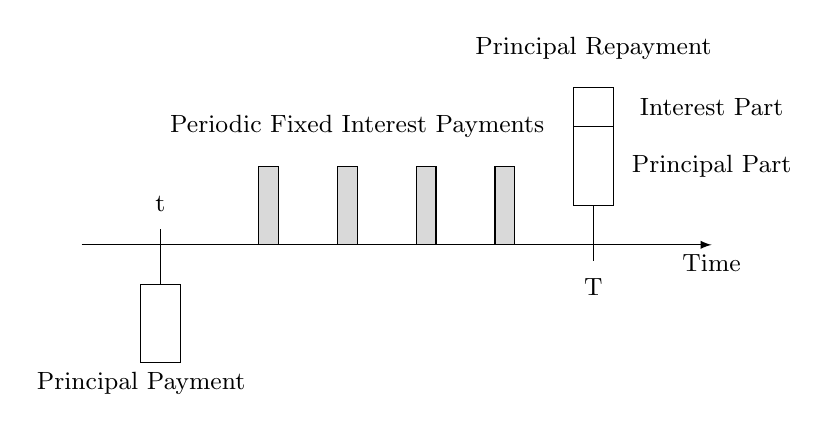
\begin{tikzpicture}[font=\small] 
        \draw[-latex] (5,0) -- (13,0) node[anchor=north] {Time};
        \draw (6,0.2) -- (6,-0.5) node[above] at (6.,0.3)  {t};
        \draw (11.5,-0.2) -- (11.5,0.5) node[below] at (11.5,-0.3) {T};
        \draw (11.75,1.5) rectangle (11.25,0.5) ;
        \draw (11.75,2) rectangle (11.25,1.5);
        \draw (5.75,-1.5) rectangle (6.25,-0.5) node[below, pos=.01] {Principal Payment};
        \draw[fill=black!15]  (10.5,0) rectangle (10.25,1);
        \draw[fill=black!15]  (8.5,0) rectangle (8.25,1);
        \draw[fill=black!15]  (9.5,0) rectangle (9.25,1);
        \draw[fill=black!15]  (7.5,0) rectangle (7.25,1);
        \node at (11.5, 2.5) {Principal Repayment};
        \node at (13.,1) {Principal Part};
        \node at (13.,1.75) {Interest Part};
        \node at (8.5, 1.5) {Periodic Fixed Interest Payments};
    \end{tikzpicture}\\[10pt] 
    Illustration 3.4: Cashflow for a fixed coupon bond
\end{center}
\subsubsection{Floating Rate Bonds}
Now a short introduction to fixed coupon bonds has been given, as mentioned there are also many 
other types of bonds that have floating coupons. When it is listed that there are bonds that have
floating coupons, what there is really said is that the rate is floating. So with the fixed coupon
bond, the coupon was predetermined when the agreement was made. But there are also bonds, where
the coupon is reset for every coupon period. These types of bonds is referred to as floating 
rate bonds. The most simple floating rate bond, is where the coupon rate $r_i$ is set to 
the spot LIBOR rate $L(T_{i-1}, T_i)$. Thus we have that 
\begin{align*}
    c_i = (T_i-T_{i-1})L(T_{i-1},T_i)K \quad \text{for} \quad i=1,...,n
\end{align*}
Here we have that $L(T_{i-1},T_i)$ is determined at time $T_{i-1}$, but the coupon is first 
delivered at time $T_i$. \cite{Bjork}  
\\\\
The LIBOR rate stands for London InterBank Offered Rate, which is a rate the the 
British Bankers Association sets every business day. Like the LIBOR rate, there is many types
of xIBOR rates, one is EURIBOR rate which is a rate the 
European Banking Federation sets every business day. 
\\\\
These different type of xIBOR rates are sets differently, but they all use the money market convention. 
So when taking about business day, the money market convention is important. This is a day-count 
convention is a standardized methodology for calculating the number of days between two dates.
This means that when $t <T_0$  the coupon dates are equally spaced with  
\begin{align*}
    \delta = T_{i}-T_{i-1}
\end{align*}
To determined the value of a the simplest floating rate bond, the LIBOR spot rate we can without
loss of generality assume that K=1 and insert Definition \ref{def:spot} of the LIBOR spot rate 
to obtain
\begin{align*}
    c_i &= (T_i-T_{i-1})L(T_{i-1},T_i)K \\
        &= \delta L(T_{i-1},T_i) \\
        &= \frac{1- p(T_{i-1},T_i)}{\delta p(T_{i-1},T_i)} = \frac{1}{p(T_{i-1},T_i)}-1
\end{align*}
Then we have found the price of the LIBOR spot rate, where $\frac{1}{p(T_{i-1},T_i)}$ is zero coupon bonds prices. 
So the next step is to determine the price for the floating rate bond. If we look at the $T_i$-payment of the floating rate bond, 
it has the value of
\begin{align*}
    P(t,T_{i-1})-P(t,T_i)
\end{align*}
If we then sum over all the i payments of the floating rate we obtain that the floating rate bond value is
\begin{align*}
    p(t)= p(t,T_n) + \sum_{i=1}^{n}\Big[p(t,T_{i-1})-p(t,T_i)\Big] = p(t,T_0) 
\end{align*}
where we note that if $t=T_0$ we get that $p(T_0)=1$ \cite{Bjork}. \\\\
Like for the section for the fixed coupon bond, a illustration of the cashflow for a floating rate bond is illustrated below.
To the to illustrations we clearly see the different in the periodic interest payments. 
\begin{center}
    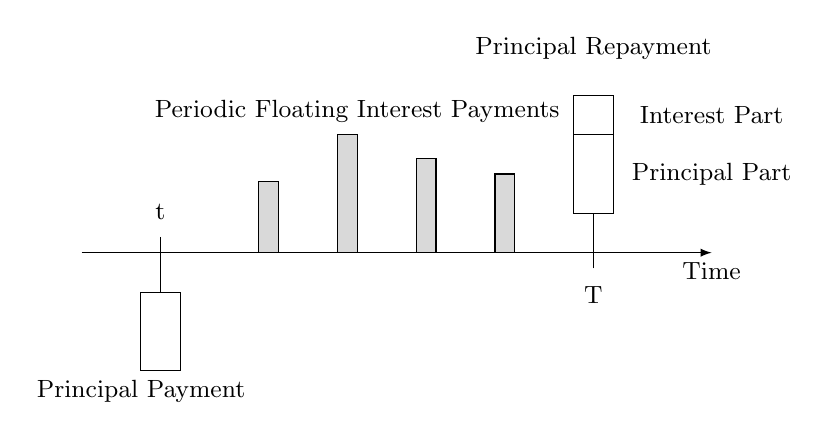
\begin{tikzpicture}[font=\small] 
        \draw[-latex] (5,0) -- (13,0) node[anchor=north] {Time};
        \draw (6,0.2) -- (6,-0.5) node[above] at (6.,0.3)  {t};
        \draw (11.5,-0.2) -- (11.5,0.5) node[below] at (11.5,-0.3) {T};
        \draw (11.75,1.5) rectangle (11.25,0.5) ;
        \draw (11.75,2) rectangle (11.25,1.5);
        \draw (5.75,-1.5) rectangle (6.25,-0.5) node[below, pos=.01] {Principal Payment};
        \draw[fill=black!15] (10.5,0) rectangle (10.25,1);
        \draw[fill=black!15]  (8.5,0) rectangle (8.25,1.5);
        \draw[fill=black!15]  (9.5,0) rectangle (9.25,1.2);
        \draw[fill=black!15] (7.5,0) rectangle (7.25,0.9);
        \node at (11.5, 2.6) {Principal Repayment};
        \node at (13.,1) {Principal Part};
        \node at (13.,1.75) {Interest Part};
        \node at (8.5, 1.8) {Periodic Floating Interest Payments};
    \end{tikzpicture}\\[10pt] 
    Illustration 3.5: Cashflow for a floating rate bond
\end{center}
\subsection{Interest Rate Swaps}
Now some simple cases of different types of bonds has be introduce. Then we will combine the knowledge we have gained to move on
to take interest rate derivatives into consideration. Again we will consider the simplest type of a interest rate derivative, which is a
interest rate swap. The construction of a interest rate swap is that there is an  exchange of a payment stream of a fixed rate of interest,
which is know as the swap rate. This fixed rate is exchanged for some floating rate, such as the LIBOR rate. 
As mentioned the fixed rate is know as the swap rate, this swap rate is determined from forward rate extracted from the yield curve, 
so it makes the present value of the swap equal to zero. This we will formulate formally later. 
\\\\
As stated in the interest rate swap, two cash flow are exchanged, where one of is a 
fixed cash flow and the other is a floating cash flow. These components of
the interest rate swap are known ad the "fixed leg" and the "floating leg". 
The role of each participant in the swap is determined in relation to the 
fixed leg: the party making fixed payments is engaged in a "payer swap," 
while the party making floating payments (and receiving fixed payments) is
involved in a "receiver swap.". The two involved cashflow there are exchanged form the "receiver" to the "payer" is illustrated below.
\\\\
\newpage
\begin{center}
    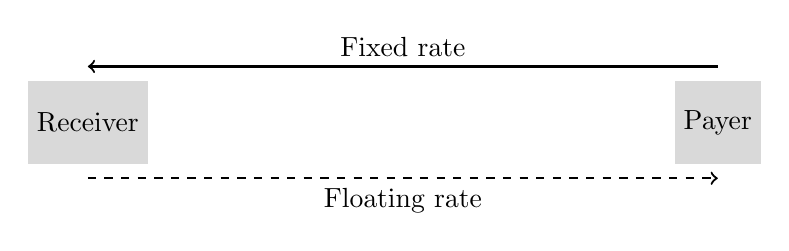
\begin{tikzpicture}
        \tikzstyle{receiver} = [rectangle, fill=black!15, text centered, minimum height=3em]
        \tikzstyle{payer} = [rectangle,  fill=black!15, text centered, minimum height=3em]
        \node[receiver] (receiver) {Receiver};
        \node[payer, right of=receiver, node distance=8cm] (payer) {Payer};
        \draw[thick, <-] ([yshift=5pt]receiver.north) -- node[above] {Fixed rate} ([yshift=5pt]payer.north);
        \draw[thick, dashed, ->] ([yshift=-5pt]receiver.south) -- node[below] {Floating rate} ([yshift=-5pt]payer.south);
    \end{tikzpicture}\\[10pt] 
    Illustration 3.6: Cashflow for fixed and floating rate exchanges
\end{center} 
\noindent
Again we have that K is the principal also know as the face value and we will denote the swap rate, R.
Further we have that payments
arises at the dates $T_1,...,T_n$, this means that at time $T_i$ the buyer of the interest rate swap will pay
\begin{align}
    K \delta L(T_{i-1},T_i)
    \label{irs}
\end{align}
where we have that $L(T_{i-1},T_i)$ is the spot rate, which could be the LIBOR spot rate.
It is also assumed
that the days $T_0,...,T_n$ is equally spaced with $\delta = T_i - T_{i-1}$ as mentioned above in the section for floating rate bonds. 
Then it is noticed that the expression in \autoref{irs} is the same as $Kc_i$, where again $c_i$ is the i'th coupon for the floating rate. 
So at time $T_i$ the buyer will pay $K \delta R$, where the cash flow at time $T_i$ is given by below
\begin{align*}
    K \delta \Big[L(T_{i-1},T_i)-R \Big]
\end{align*}
Then by applying the results from the section for floating rate bonds again, we are able to compute the value of the 
cash flow at time $t<T_0$. The value of the cash flow is listed below
\begin{align*}
    K p(t,T_{i-1})-K(1+\delta R)p(t,T_i)
\end{align*}
Hence we have that the total value denote by $\Pi(t)$, so the total value at time t of the swap is given as below
\begin{align}
    \pi (t) = K \sum_{i=1}^{n} \Big[p(t,T_{i-1})-(1+ \delta R)p(t,T_i)\Big]
    \label{valueirs}
\end{align}
Moving forward we simplify \autoref{valueirs} in the below Proposition \ref{simple} \cite{Bjork}.
\begin{proposition}
    The price, for $t<T_0$, of the swap in \autoref{valueirs} above
    is given by 
    \begin{align*}
        \Pi(t) = K p(t,T_0)-K \sum_{i=1}^{n}d_i p(t,T_i)
    \end{align*}
    where
    \begin{align*}
        d_i &= R \delta, \quad i=1,...,n-1 \\
        d_n &= 1+ R \delta
    \end{align*}
    \label{simple}
\end{proposition}
\noindent 
To sum up on interest rate swaps, let consider a timeline for a payer swap contract. Where the issuer is paying the fixed leg 
and receiving the floating leg. The timeline of the contract is illustrated below, where a time t the contract is made. 
Then the swap start a time $T_S$ and maturities at time $T_E$.
The squiggly lines denote the floating interest payments that the payer will make based on the interest rate observed 
at the beginning of the period and the end of the period. The vertical lines at the beginning of each period represent
the fixed payment dates, and the horizontal dotted line indicates the continuation of the swap contract over time.
\begin{center}
    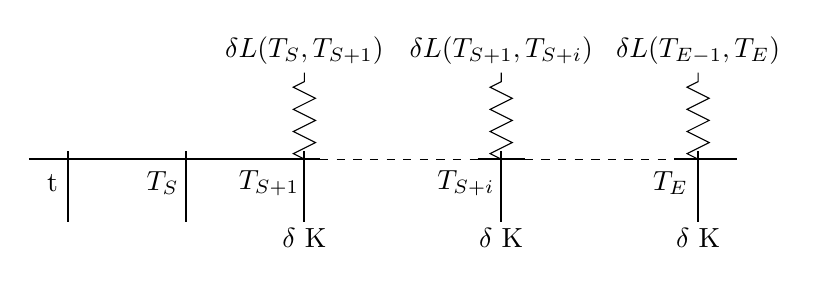
\begin{tikzpicture}
        \draw[thick] (0,0) -- (3.7,0);
        \draw[dashed](3.7,0) -- (5.7,0);
        \draw[thick] (5.7,0) -- (6.3,0);
        \draw[dashed](6.3,0) -- (8.2,0);
        \draw[thick] (8.2,0) -- (9.0,0);
        \draw[thick] (0.5,0.1) -- (0.5,-0.8) node at (0.3,-0.3) {t} ;
        \draw[thick] (2,0.1) -- (2,-0.8) node at (1.7,-0.3) {$T_S$} ;
        \draw[thick] (3.5,0.1) -- (3.5,-0.8) node at (3.05,-0.3) {$T_{S+1}$} ;
        \draw[thick] (6.0,0.1) -- (6.0,-0.8) node at (5.55,-0.3) {$T_{S+i}$} ;
        \draw[thick] (8.5,0.1) -- (8.5,-0.8) node at (8.15,-0.3) {$T_{E}$} ;
        \draw[decorate, decoration={zigzag, segment length=8pt, amplitude=4pt}] (3.5,0) -- node[above=15pt] {$\delta L(T_{S}, T_{S+1})$} (3.5,1.1);
        \draw[decorate, decoration={zigzag, segment length=8pt, amplitude=4pt}] (6,0) -- node[above=15pt] {$\delta L(T_{S+1}, T_{S+i})$} (6,1.1);
        \draw[decorate, decoration={zigzag, segment length=8pt, amplitude=4pt}] (8.5,0) -- node[above=15pt] {$\delta L(T_{E-1}, T_{E})$} (8.5,1.1);
        \node at (3.5,-1.) {$\delta$ K};
        \node at (6,-1.) {$\delta$ K};
        \node at (8.5,-1.) {$\delta$ K};
    \end{tikzpicture}\\[10pt] 
    Illustration 3.7: Cashflow for a payer swap 
\end{center}
Earlier we left behind a discussion of how the swap rate, R,  is determined. 
It was noted that the swap is determined such that the present value of
the swap is equal to zero. Now we will give a more accurate definition of how swap rates is determined in Proposition \ref{swaprate1}.
\begin{proposition}
    If, by convention, we assume that the the contract is written at $t=0$, 
    the swap rate is given by \cite{Bjork}
    \begin{align*}
        R = \frac{p(0,T_0)-p(0,T_n)}{\delta \sum_{i=1}^{n}p(t,T_i)}
    \end{align*} 
    \label{swaprate1}
\end{proposition}
\noindent 
If we have that $T_0=0$ the formula for the swap rate, R, becomes
\begin{align*}
    R= \frac{1-p(0,T_n)}{\delta \sum_{1}^{n}p(0,T_i)}
\end{align*}
\subsection{Options}
In this section will introduce the framework of options in the over-the-counter-market. 
The purpose of this section is to establish a pricing formula for European call options.
The meaning of introducing pricing of options before introducing swaptions pricing, is that a swaption is  a 
more complex derivative. So the idea is to get a fundamental understanding of pricing derivatives in a more simple case.
\\\\
Firstly, let's clarify what the over-the-counter market (OTC) is. It is  a marketplace where numerous trades occur.
In the OTC market private companies exchange trades, these companies are firms as banks, other 
large financial institutions and funds managers \cite{Hull}. Then we have established the market where 
options is traded, so moving forward we will look in to options contracts. 
\\\\
A call options gives the holder the right to buy the underlying asset at a fixed strike price, K, at a 
predetermined time, T. Where a put option gives the holder the right to sell the underlying asset at a fixed
strike price, K, and a predetermined time, T. Options contracts come in various types, with the 
most common being the European and American options, followed by Bermudan options. European options can only 
be exercised at the maturity date, while American options can be exercised at any time point upon to the maturity date.
Bermudan options allow exercise at specific predetermined time points.
For the purpose of understanding the basics of options pricing, we will focus on the European option. 
The contract functions, $\Phi$, for European call and put options are as follows.
\begin{align}
    \Phi(x)_{\text{call}} &=  \max[S-K,0] \label{call_function}\\ 
    \Phi(x)_{\text{put}} &= \max [K-S,0] \label{put_function}
\end{align}
where K is the strike price, S denotes the market price of the underlying asset \cite{Bjork}. From \autoref{call_function} and \autoref{put_function} we see
that the value of the contract function can not be negative, since in both cases the contract function is a 
function there takes the maximum of the payoff and zero. So the holder maximum lost is the paid premium. Below the described contract
function for a European call option is illustrated.
\begin{center}
    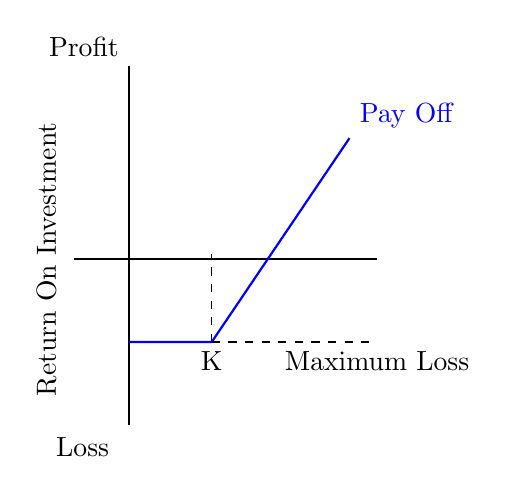
\begin{tikzpicture}[scale=0.7]
        \draw[thick] (-1,0) -- (4.5,0) ;
        \draw[thick] (0,-3) -- (0,3.5) node[anchor=south east] {Profit};
        \coordinate (K) at (1.5,-1.5);
        \draw[dashed] (K) node[below] {K} -- ++(0,1.6);
        \draw[thick, blue] (0,-1.5) -- (K) -- (4,2.2) node[anchor=south west] {Pay Off};
        \draw[dashed] (1.5,-1.5) -- (4.5,-1.5) node[below] {Maximum Loss};
        \draw (-1.5,-3.4) node[anchor=west] {Loss};
        \node[rotate=90] at (-1.5,0) {Return On Investment};
    \end{tikzpicture}\\[10pt] 
    Illustration 3.8: Contract function for a European call option
\end{center}
\subsubsection{Risk Neutral Measure} \label{risk_neutral_section}
Before options pricing a brief introduction to the risk neutral measure will be covered.
When options are priced the value of the options is calculated by discounting 
the options expected payoff at time T under the risk neutral measure $\QQ$. 
\\\\
The value of the options is calculated under the risk neutral measure $\QQ$ also know as the pricing measure, and 
not under the actual measure $\PP$. The $\PP$- measure reflects th real world probabilities. If prices was determined 
under $\PP$ is could lead to arbitrage opportunities, because it would reflect the actual risk preferences of
investors, who demand different rates of return for different risks. Under the risk neutral measure $\QQ$  
probabilities are shifted or adjusted in such way that the expected rate of return on assets becomes the risk-free rate. 
This adjustment removes the risk premiums that are present in the actual probability measure $\PP$.
This lead to the First Fundamental Theorem of Asset Pricing, to develop this theorem we consider 
the concept of martingales. 
A stochastic process $X_t$ is a $\QQ$-martingale, if the process has no drift term (dt-term). Which is satisfied if it holds that
$\EE_{t}^{\QQ}\Big[X_T\Big] = X_t$ for all $t<T$. Next we will consider a price process $X_t$ with the following dynamic.
\begin{align}
    d X_t = r_t X_t dt + \sigma X_t d W_{t}^{\QQ}
    \label{price_process}
\end{align}
where $W_{t}^{\QQ}$ is $\QQ$-Wiener process and  $r_t$ is the process for the risk free interest rate. $r_t$ can be looked at the locally risk-free rate return 
from a continuously compounded bank account $B(t)= \text{exp} \Big[\int_{0}^{t}r(s)ds \Big]$.
Where the bank account has the following dynamic
\begin{align}
    dB(t) &= r(t)B(t) dt \label{bank1}\\
    B(0) & = 1 \label{bank2}
\end{align}
If we look at \autoref{price_process} we see there is a dt-term present, so it is not a martingale.
But if we discount the price process, this will be a martingale do to the martingale property below
\begin{proposition}
    (\textbf{The Martingale Property}) In the Black-Scholes model, the price process $\Pi_t$
    for every traded asset, be it the underlying or derivative asset, has the property that the normalized price process
    \begin{align*}
        Z_t = \frac{\Pi_t}{B_T}
    \end{align*}
    is a martingale under the measure $\QQ$ \cite{Bjork}
\end{proposition}
\noindent 
This lead os to the First Fundamental Theorem of Asset Pricing in \autoref{frist_theorem_of_asset_pricing}.
\begin{theorem}
    (\textbf{First Fundamental Theorem of Asset Pricing})
    Given a time horizon, a risky asset with price process $X_t$ and a
    risk-free asset with price process $B_t$, the market is arbitrage free 
    (under the probability measure $\PP$) if and only if there exists an 
    equivalent probability measure $\QQ$ such that the discounted price process
    $\Big[\frac{X_t}{B_t}\Big]$  is a $\QQ$- martingale \cite{Bjork}
    \label{frist_theorem_of_asset_pricing}
\end{theorem}
\noindent 
Hence we have establish the First Fundamental Theorem of Asset Pricing. So to sum up in order to be able to calculate
option prices, the "fair" or arbitrage-free price, there must exist a risk neutral measure $\QQ$, such the the discount prices
is a $\QQ$-martingale. 
\subsubsection{Options Pricing}
The next question to be answered is what is the "fair" price of these options, we will denote the price of
the option by $\Pi(t)$. Again to simplify we will consider
the European call option moving forward. To determine the price of a European call potion, we wil use the 
Black-Scholes formula. This requires a review of Risk Neutral Valuation and the Black-Scholes model.
\\\\
Risk Neutral Valuation determine the value of an asset by discounting the expected values of the assets future 
pay-offs at the risk-free rate of return, this formalized in \autoref{rnt} below
\begin{theorem}
    \textbf{(Risk Neutral Valuation)} The arbitrage free price of the claim $\Phi(S_t)$ is given by \\
    $\Pi(t)[\Phi]$=$F(t,S_t)$, where F is given by the formula 
    \begin{align*}
        F(t,s) &= -e^{-r(T-t)} \EE_{t,s}^{\QQ} \Big[\Phi(S_T)\Big]
    \end{align*}
    where the Q-dynamics os S is
    \begin{align*}
        dS_t & = r S_t dt + S_t \sigma(t,S_t) dW^{\QQ} \\
        S_0 & = s
    \end{align*}
    and $W^{\QQ}$ is a $\QQ$-Wiener process \cite{Bjork}
    \label{rnt}
\end{theorem}
\noindent 
The Risk Neutral Valuation has been introduced, hence the only thing left before we are able to price a 
European call option, is to establish the model the price in found under. In this case it is the Black-Scholes model.
It consists of two asses, a risk free asset with price process, B, and a stock price with price process, S.
The dynamics of the two assets is listed below
\begin{align*}
    dBt & = rB_t dt \\
    dS_t &= \mu S_t dt + \sigma S_t dW_t
\end{align*}
where the short rate, r, is  a deterministic constant,  $\mu$ and $\sigma$ is two constants. It is also assumed
that the stock price process is lognormal distributed. From \autoref{rnt}
(Risk Neutral Valuation) the formulas for determine the arbitrage free price is available. Finally the requirements
for being able to price a European option is satisfied, hence we have the Black-Scholes Formula below.
\begin{proposition}
    \textbf{(Black-Scholes Formula)} The price of a European call option with strike K and time of maturity T 
    is given by the formula $\Pi$ = $F(t,S_t)$
    \begin{align*}
        F(t,S_t) & =s N[d_1(t,s)] -e^{-r(T-t)}KN[d_2(t,s)] 
    \end{align*}
    Here N is the cumulative distribution function for the N $[0,1]$ distribution and 
    \begin{align*}
        d_1(t,s) &= \frac{1}{\sigma \sqrt{T-t}} \Big[ \ln \Big(\frac{s}{K} \Big) +  \Big(r + \frac{1}{2} \sigma^2)(T-t)  \Big] \\
        d_2(t,s) &= d_1(t,s)-\sigma \sqrt{T-t}
    \end{align*}
    \label{Black-Scholes Formula}
    \cite{Bjork}
\end{proposition}
\subsection{Swaptions}
Now that we have establish a foundational understanding of interest rates, bonds, swaps and options, we can
now go deeper into swaptions. First we will explain what constitutes a swaption and the we will continuing 
to develop the framework of pricing a swaption, buibuiltld on the knowledge we have established.  
\\\\
A swaption is a financial derivative that can be describeed as an option to exchange a fixed rate bond for
floating rate bonds for a predetermined principal. 
There are two types of swaptions, payer swaptions and receiver swaptions.
A payer swaption gives the holder the right to pay a fixed interest rate and receive a floating rate, 
similar to a call option in the stock market. On the other hand, a receiver swaption allows the holder
to pay a floating interest rate and receive a fixed rate, resembling a put option \cite{Lindstrom} .

\subsubsection{Swaption Pricing}
Swaptions pricing purpose is to calculating the present value of expected payments from the swap contract,
should the option be exercised. The pricing model must take various factor into account, such as the
volatility of interest rates, the term structure of interest rates, and the time value of money. 
To price swaptions, the Black model will be used, which is an extension of the Black Scholes
model for equity options. The choice of using the Black model for pricing swaption is commonly used, especially when
is purpose is the price European swaption. Likewise for swaps, there is also different type of swaptions. 
Again European options can only be exercised at the maturity date, while American options can be exercised
at any point in time up to the maturity date. Moving forward we will only consider European swaptions. 
The Black model assumes that the underlying swap rate follows a lognormal distribution and uses a 
risk neutral valuation approach. These concept has been reviewed earlier, hence we can the move on to 
formulating pricing swaptions.
\\\\
First we consider a swaption that is settled such that the holder has the right to pay a fixed rate, $S_K$, 
and receive a floating rate on the swap that will expire in n year starting in T years.
Further we will assume that there are m payments 
per year under the swaption and we will let the notional principal be denoted by L. These m payments has
assumed that each fixed payment on the swap is the fixed rate times L/m. Next we suppose that 
the given swap rate for an n-year swap staring a time T, is denoted by $S_T$. 
From the knowledge on swaps we formulate the payoff function of the swaption, which is listed in
\autoref{swaptionspay} below
\begin{align}
    \frac{L}{M} \max \Big( S_T - S_K, 0 \Big)
    \label{swaptionspay}
\end{align}
We note that the cashflow generated from the payoff function of the swaption, is reviewed m times 
a year. The most commonly frequency payments is semi-annually and annually. These payments at m times
of a year, is paid throughout the life of the swap. The payment of the swap, have the following 
payments dates 
\begin{align*}
    T_1,T_2,...,T_{mn}
\end{align*}
Let us be reminded that a swaption is a option on the swap rate, which is the one that generated the payoffs.
Then we formulated the price of the payer swaption as \cite{Hull}
\begin{align*}
    \Pi(t)_{\text{Payer swaption}} = \sum_{i=1}^{mn} \frac{L}{m} p(0,T_i)\Big[ S_F N(d_1) - S_K N(d_2)\Big] \quad \text{for} \quad T_i= T+i/m  
\end{align*}
where
\begin{align*}
    d_1 & = \frac{1}{\sigma \sqrt{T}} \Big[ \ln \Big(\frac{S_F}{S_k}\Big)+\sigma^2\Big(\frac{T}{2}\Big)\Big] \\
    d_2 & = d_1-\sigma \sqrt{T}
\end{align*}
Where N is the cumulative distribution for the $N [0,1]$ distribution, $S_F$ is the forward swap rate a time
zero, $\sigma$ is the volatility of the forward swap rate. The term $\sum_{i=1}^{mn} \frac{L}{m} p(0,T_i)$ 
is the discount factor for the mn payoffs. To simplify we define A as the values of the contract that
pays $1/m$ at times $T_i ( 1\leq i \leq mn)$ a in \autoref{a_simple}
\begin{align}
    A= \frac{1}{m} \sum_{i=1}^{mn} p(0,T_i)
    \label{a_simple}
\end{align}
Hence we have that the value of the swaption can be expressed as 
\begin{align*}
    L N \Big[S_F N(d_1) - S_K N(d_2) \Big]
\end{align*}
Which leads to the case we looked at, where the contract of the swaption was made such that the 
holder has the right to receive a fixed rate of $S_K$ instead of paying it. It also leads to
the payoff of the swaption as listed in \autoref{payoff_swaption} below. We note that the payoff 
is a payoff function of a put option on $S_T$. 
\begin{align}
    \frac{L}{M} \max \Big( S_K - S_T, 0 \Big)
    \label{payoff_swaption}
\end{align}
Finally we can end this section with the value of a swaption in a standard market model \cite{Hull}.
\begin{align*}
    \Pi(t)_{\text{swaption}}= L A \Big[S_K N(-d_2) - S_F N(-d_1)\Big]
\end{align*}
To summarize the mathematics of pricing a swaption has been reviewed, which include introducing interest rates, 
bonds, swaps and option. It is important to remember which choices was made along the way,
because the price of the swaption depends on the choice of the model. But now the simplest case has been 
introduced, so we can move forward with the analysis. 